\chapter{Optimal Motion Planning for Humanoid Robots}
\label{chap:optimal-motion-planning}

This paper aims at combining state of the art developments of path
planning and optimal control and to create the algorithmic foundations
to tackle optimal control problems in cluttered environments. Our
contribution is three-fold: first, we describe a simple method to
automatically generate minimum bounding capsules around exact robot
body geometries represented by meshes. Second, we use the bounding
capsules to implement distance constraints for an optimal control
problem solver and achieve (self-)collision avoidance. Finally, we
propose a complete two-stage framework for optimal motion planning on
complex robots. This framework is successfully applied to generate
optimal collision-free trajectories both in simulation and on the
humanoid robot HRP-2.

\section{Introduction}
The generation of the best possible trajectory that does not violate
any constraints imposed by the environment is an ubiquitous task in
both industrial and humanoid robotics. Numerous examples of successful
robotic applications in the domains of motion planning and optimal
control can be encountered in literature and industry. Very few
however, if none, consider the more general problem of optimal motion
planning for complex robots evolving in complex environments.

This paper aims at combining state of the art developments of these
two domains and to create the algorithmic foundations to tackle
optimal control problems in cluttered environments.

\section{Related Work}
There are two established but still quite separate research areas that
both address a part of the optimal motion planning problem, namely
path planning and numerical optimal control.

\subsection{Path Planning}
Let the configuration \config{} be a vector containing the generalized
coordinates of a robot, and let \cspace\enspace be the set of all
possible configurations \config{}. Path planning is mainly interested
in the determination of a feasible path $P$ connecting a start
configuration \config{s} to a goal configuration \config{g} in
\cspace. $P$ is said to be feasible iff for all \config{} $\in
P$, \config{} is valid with respect to both geometric constraints,
e.g. (self-)collision avoidance, and kinematic constraints of the
robot, e.g. joint limits.

Sampling-based algorithms, such as Rapidly-exploring Random Trees
(RRT) \cite{kuff00}, are particularly powerful when it comes to
solving path planning problems in high-dimension \cspace\thinspace and
cluttered environments. In its simplest form, this algorithm expands a
tree \ctree rooted in \config{s} by first sampling a random
configuration \config{rand} in \cspace, then extending a valid edge
from the nearest configuration \config{near} in \ctree towards
\config{rand}. This process is repeated until \ctree and \config{g}
can be connected.

%% Keep for next paragraph
%% Such is the case for robots with a floating base, i.e. the
%% configuration contains an unactuated part that can be changed only
%% through maintaining contact with the environment.

It is interesting to note that all nodes and edges of the final tree
\ctree lie in \cspace. This can lead to infeasible paths if the robot
must respect additional kinematic constraints. \cite{dali09,
  berenson09, stilman2007tcm} propose variants of RRT where the
extension phase produces an edge that lies in its entirety on a
manifold $\manifold$ of \cspace. $\manifold$ is defined by kinematic
constraints, each defined by a feature value in the operational space,
e.g. end-effector position and orientation. The constrained RRT
algorithm produces a path $P$ such that for all \config{} $\in P$,
\config{} lies on the manifold $\manifold$.

An important feature of sampling-based algorithms is their
probabilistic completeness, i.e. their capacity to avoid falling into
local minima and to find a solution path if it exists. They present
however three drawbacks. First, due to their sampling nature, the
configuration \config{} might move in a random fashion along the path
$P$, which could lead to unnecessarily long and unnatural
paths. Second, we still need to apply a time parametrization in order
to transform the path into a trajectory. This is a non-trivial task in
the particular case of a humanoid robot, as we must ensure its dynamic
balance along the trajectory. Third, the resulting paths are
continuous but not $C^1$. The time-parametrized motion thus needs to
stop at each waypoint or to leave the planned path around waypoints.
Additional processing is thus needed to provide a reshaped
collision-free trajectory that can be executed on the robot.

\subsection{Numerical Optimal Control}
Given a dynamic model, let:
\begin{itemize}
\item $t$ be the time variable,
\item \state{} be the state vector, 
\item \control{} be the control vector,
\item $t_f$ be the trajectory duration,
\item $\phi$ be the scalar objective function to minimize,
\item \dfcn{} be the differential equation of the model,
\item \eqcstr{} be the equality constraint vector function,
\item \ineqcstr{} be the inequality constraint vector function,
%\item \bndcstr{} be the boundary conditions vector function. 
\end{itemize}

An optimal control problem can be written as follows:

\label{OCP}
\begin{equation}
  \min_{x (\cdot), u (\cdot), t_f} \ \ 
  \int_{0}^{t_{f}}\phi (x(t), u(t))dt
  \label{OCP:Obj}
\end{equation}
\ \ \ subject to:

\begin{equation}
  \begin{array}{rcl}
  \dot{x} (t) & = & f(t, x(t), u(t)) \label{OCP:Model}
  \\
  g(t, x(t), u(t)) & = & 0,
  \\
  h(t, x(t), u(t)) & \ge & 0%,
  \\
  %% r (x (0), x (t_{f})) & = & 0.
  %% \\
  \end{array}
\end{equation} 

Starting from an initial value of \state{} and \control{}, numerical
optimal control techniques are capable of iteratively converging
towards a trajectory that locally minimizes $\phi$ while taking into
account the dynamics of the system and verifying equality and
inequality constraints given by Eq. \ref{OCP:Model}.

There exists several classes of optimization solvers, among which
gradient-based methods such as interior point optimizers implemented
notably in IPOPT \cite{Biegler2009}, and Sequential Quadratic Program
(SQP) solvers. Particularly, multiple shooting optimization,
implemented in the \textsc{MUSCOD-II} software \cite{Leineweber2003},
is a powerful tool that allows solving large-scale optimal control
problems thanks to a specially tailored SQP.

Note that for all gradient-based solvers, the objective and constraint
functions can be nonlinear, but they must be at least $C^1$,
i.e. continuously differentiable. This requirement can be alleviated
by the use of non gradient-based solvers such as STOMP
\cite{Kalakrishnan2011}, but this method has so far been only applied
to simple trajectory optimization problems where obstacle and torque
constraints were integrated in the cost function.

%, which can be a non-trivial task in complex environments,

Optimal control techniques have been successfully applied on humanoid
figures \cite{Schultz2010} and humanoid robots \cite{Toussaint2007,
  Lengagne2010}. The problems take into account complex robot dynamics
and actuator limitations. However, current formulations either work
under the assumption that the initial guess is collision-free or allow
it to be slightly in collision by means of linear interpolation
between initial and final configurations. There are then cases where
the solver might get stuck in local minima and fail to generate a
trajectory without any collisions with either the environment or
bodies of the robot. Hence, initial trajectory generation and
collision avoidance have yet to be treated properly in the optimal
control formulation.

\subsection{(Self-)Collision Avoidance Constraints}
There are several ways to express collision avoidance constraints
between two bodies; one can express the constraint with the exact
distance between the exact polyhedral geometries such as in
\cite{Larsen2000}. While distance computation is precise and efficient
thanks to bounding volume hierarchy structures, distance is zero in
case of penetration, which forbids the computation of a correct
constraint gradient. \cite{Kim2002} propose a fast penetration
computation algorithm, but computation times are
restrictive. Moreover, the distance constraint between two
non-strictly convex polyhedra is not $C^1$, which can cause the
optimization solver to behave incorrectly. \cite{Escande2007} proposes
a nice solution to this problem and introduces Sphere-Torus Patches
Bounding Volumes (STPBV), which are strictly convex bounding volumes;
in this case the distance between a STPBV and a convex mesh is always
$C^1$. These constraints are successfully used for self-collision
avoidance in real-time control of a humanoid robot
\cite{Stasse2008}. In \cite{Kanoun2011}, also in a control context,
self-collision constraints are expressed as the distance between
bounding capsules, i.e. cylinders capped by half-spheres.

\subsection{Sampling-Based Optimal Motion Planning}

Recently \cite{Karaman2011} introduced RRT*, a new variant of RRT that
has the property of asymptotically converging towards the global
minimum solution path. This is a very interesting approach as only one
algorithm is needed to achieve optimal motion planning. But if we want
to generate an optimal trajectory, we need to explore not only the
configuration space \cspace, but the whole state space
\sspace\thinspace where an element of \sspace\enspace is \state{} =
$[$\config{}$,$ \dotconfig{}$]^T$. This doubles the dimension of the
problem. Another problem arises from choosing the correct metric and
local optimal policy. \cite{Perez2012} propose a variant uses local
linearization of a system to derive a coherent extension
method. Results have so far been only obtained on simple systems, and
this method has yet to be tested on complex ones.

\section{Contribution}
To the authors' best knowledge there is no available algorithmic
approach that addresses the problem of optimal motion planning for
complex robot systems in cluttered environments.

Our contribution is three-fold: first, we describe a simple method to
automatically generate minimum bounding capsules around exact robot
body geometries. Second, we use the bounding capsules to implement
distance constraints for the solver and achieve (self-)collision
avoidance. Finally, we propose a complete two-stage framework for
optimal motion planning on complex robots. Given a start and goal task
or configuration, the constrained path planner produces a
collision-free path where kinematic constraints have been enforced,
thus avoiding geometric local minima. This path is given as an initial
guess to the \textsc{MUSCOD-II} solver, which generates a locally
optimal trajectory while enforcing dynamic constraints and
(self-)collision avoidance. This framework is successfully applied to
generate optimal collision-free trajectories both in simulation and on
the humanoid robot HRP-2.

Section \ref{path-planning} describes the path planning stage. The
collision avoidance constraints are tackled in section
\ref{distance-constraints}, and are used in the optimal control
problem described in section \ref{framework}. Finally, section
\ref{results} showcases results on the robot HRP-2.

\section{Constrained Path Planning}
\label{path-planning}

\begin{figure}
\centering
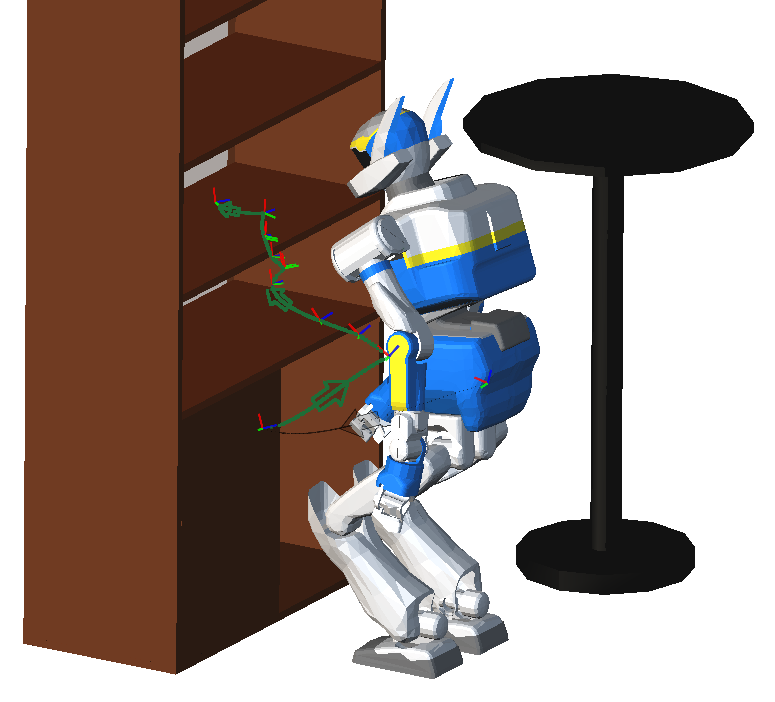
\includegraphics[width=0.8\linewidth]
                {src/chap3-optimal-motion-planning/figure/shelves-path.png}
\caption{Path found by the path planner in a shelves environment.}
\label{path}
\end{figure}

We use the constrained planner in \cite{dali09}, which is
implemented with the motion planning library KineoWorks\texttrademark
\cite{Laumond2006}. This planner allows generating a collision-free
path, while guaranteeing that the solution path lies on a manifold of
the configuration space. We want to generate for HRP-2 a
collision-free path that guarantees its quasi-static balance when it
is standing on both feet. We then define the manifold $\manifold$
with the following stack of equality constraints:

\begin{enumerate}
  \item Right foot has a fixed 6D transformation,
  \item Left foot has a fixed 6D transformation,
  \item Center of mass vertical projection lies in the center of the
    support polygon.
\end{enumerate}

Additionally, we would like to avoid choosing a single goal
configuration \config{g}, but instead define a goal task
\task{g}. This task can be defined by a sub-manifold
$\goalmanifold$\thinspace of the planning manifold $\manifold$. For a
simple object manipulation task, $\goalmanifold$\thinspace can be
defined as the intersection between $\manifold$\thinspace and the
manifold defined by the following stack of equality constraints:

\begin{enumerate}
  \item Gripper has the same 3D position as the object to grab.
  \item Gripper thumb is oriented vertically.
\end{enumerate}

Given a start configuration \config{s} a planning manifold $\manifold$
and a goal sub-manifold $\goalmanifold$, we first create a set of goal
configurations \config{g} by sampling a fixed number of configurations
in $\goalmanifold$, then we solve the path problem from \config{s} to
\config{g}. The constrained planner diffuses trees from \config{s} and
each configuration of \config{g}, and stops once at least one of the
goal configurations is in the same connected component as
\config{s}. A shortcut optimizer can then prune unnecessary waypoints
and smooth the solution path. Figure \ref{path} shows an example where
HRP-2 has to grab an object on the lower shelf and place it on the
upper shelf.

\section{(Self-)Collision Avoidance Constraints}
\label{distance-constraints}
In path planning, Boolean collision queries are used to validate or
invalidate configurations and hence the whole path. This is not enough
in optimal control, especially for gradient-based solvers where
constraint must be $C^1$. Furthermore we need to return negative
values of the distance in case of collision to provide the solver the
means to get out of collision.

We choose to use bounding capsules, like in
\cite{Kanoun2011}. Capsules are sphere swept segments; the
inter-capsule distance can be simply found by computing the distance
between the capsule axes, then subtracting their radii. Similarly, we
can compute the distance between a capsule and a polyhedron by
computing the distance between the capsule axis and the polyhedron,
then subtracting the radius. The returned distance can then become
negative in case of collision.

\subsection{Computing minimum bounding capsules}
In \cite{Kanoun2011}, bounding capsules parameters, i.e. the 2
endpoints $\mathbf{e_1}, \mathbf{e_2}$ and the radius $r$, were set by
hand to obtain the best fitting capsules around the body
geometries. We propose here to automatically find these parameters by
solving, offline and once for each body of the robot, the following
optimization problem:

\begin{equation}
  \min_{\mathbf{e_1}, \mathbf{e_2}, r} \ \ 
  \|\mathbf{e_2} - \mathbf{e_1}\| \pi r^2 + \frac{4}{3}\pi r^3
  \label{capsule-objective}
\end{equation}
\ \ \ subject to:
\begin{equation}
  \begin{array}{rcll}
    r - d(\mathbf{p},\mathbf{e_1e_2}) & \ge & 0\mbox{, for all }
    \mathbf{p} \in \mathcal{P}
    \label{capsule-constraint}
  \end{array}
\end{equation} 
where $d(\mathbf{p},\mathbf{e_1e_2})$ is the distance of $\mathbf{p}$
to line segment $\mathbf{e_1e_2}$.  Equations \ref{capsule-objective}
and \ref{capsule-constraint} mean we want to find the minimum-volume
capsule while ensuring all points $p$ of the underlying polyhedron
$\mathcal{P}$ lie inside the capsule. HRP-2 has 41 bodies, each body
polyhedron containing about 1000 points. We solve all 41 optimization
problems with RobOptim \cite{roboptim, moulard2012optimisation} and
the IPOPT solver \cite{Biegler2009} in less than 5s. Figure
\ref{hrp2-capsule} shows the best fitting bounding capsules
superimposed on the robot geometries.

FIXME: Add figure with romeo, kuka, hrp2.

\begin{figure}
  \centering
  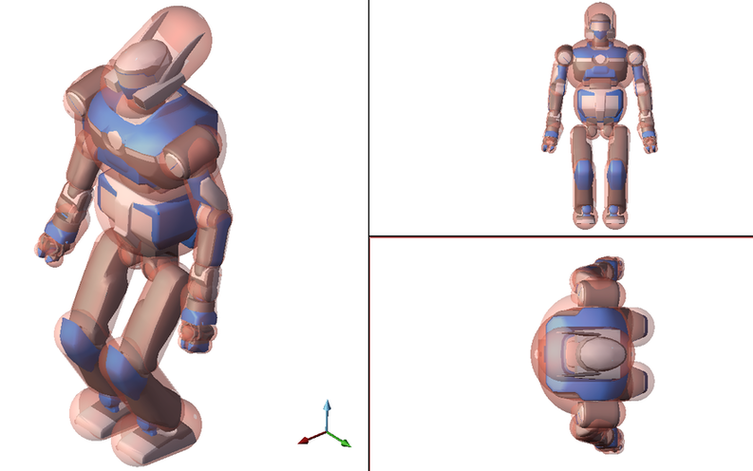
\includegraphics[width=0.9\linewidth]
                  {src/chap3-optimal-motion-planning/figure/hrp2-capsule-transparent.png}
  \caption{Best fitting capsules for HRP-2}
  \label{hrp2-capsule}
\end{figure}

\subsection{Distance computation}
As mentioned previously, for capsule-capsule distance pairs, we need
to compute the distance between the two capsule axes then subtract the
radii to obtain the real distance. We rely on the Wild Magic geometric
library \cite{schneider2003geometric, wildmagic} to compute this
distance in an average time of 2 $\mu$s.

Concerning capsule-polyhedron pairs, we rely on an implementation of
OBB-Trees in the Kineo Collision Detection (KCD) library
\cite{Laumond2006} for an efficient computation. For the environment
in figure \ref{path}, the distance for one capsule-environment pair
takes about 500 $\mu$s to be computed, since the environment is
assumed to be perfectly modeled by polyhedron meshes.

\subsection{Selection of pairs of bodies for distance computation}
If we take into account all capsule-capsule pairs of the robot, we end
up with $\frac{n(n - 1)}{2}$ possible pairs, with $n$ the number of
bodies. This means that for a robot like HRP-2, we can have up to 820
pairs and it can be very costly to evaluate the distance for all of
them. Luckily, some bodies are either always colliding because they
are adjacent in the kinematic tree, or never colliding due to the
joint limits; the pairs corresponding to those bodies can be safely
pruned. We use the tool described in \cite{planning-environment},
which relies on finely exploring the configuration space and keeping
track of colliding bodies, to save 510 useful pairs. Furthermore,
since we are in the particular case of double-support motion, we can
be sure that most of the leg bodies cannot collide with each other due
to the additional kinematic constraints. We finally end up with 327
capsule-capsule pairs that must be all evaluated to guarantee
self-collision avoidance. Similarly, we can prune some of the 41
capsule-environment pairs that do not need to be checked due to the
particular kinematic structure of the HRP-2. For instance, if both
waist and chest are not in collision with the environment, we can be
sure that it will be the same for the intermediate body linking
them. We thus keep 23 capsule-environment pairs.

\section{Description of Optimal Motion Planning Framework}
\label{framework}

Now that we have properly set distance pairs, we can establish a
complete formulation of the optimal control problem for the second
stage of our optimal motion planning framework.

\subsection{Optimal Control Problem Formulation}

\subsubsection{Objective function}

We choose to minimize, for a fixed duration, the integral over time of
the sum of square jerks, as this criterion leads to smooth and natural
trajectories.

The objective function can then be written as:
\begin{equation}
  J = \int_{0}^{t_{f}}\mathbf{\dddot{q}}(t)^T\mathbf{\dddot{q}}(t) dt
  \label{objective-function}
\end{equation}

and we define the state and control variables to be:
\begin{equation}
  \begin{array}{rcl}
  \mathbf{x}(t) & = & [\mathbf{q}(t), \mathbf{\dot{q}}(t), \mathbf{\ddot{q}}(t)]^T \\
  \mathbf{u}(t) & = & [\mathbf{\dddot{q}}(t)]^T
  \end{array}
  \label{variables}
\end{equation}

\subsubsection{Equality and inequality constraints}

\paragraph{Joint constraints}
% and mechanical structure
Each actuated joint is subject to physical limitations of its
underlying actuator. Box constraints on angular, speed and torque
limits are then added as:

\begin{equation}
  \begin{array}{rcccl}
    \mathbf{q_{min}} & \le & \mathbf{q} & \le & \mathbf{q_{max}} \\
    \mathbf{\dot{q}_{min}} & \le & \mathbf{\dot{q}} & \le & \mathbf{\dot{q}_{max}} \\
    \mathbf{\tau_{min}} & \le & \mathbf{\tau} & \le & \mathbf{\tau_{max}}
  \end{array}
  \label{joint-constraints}
\end{equation}

\paragraph{Dynamic balance}
The robot is submitted in our case to multiple coplanar contact
reaction forces from the ground. We can then express the dynamic
balance constraint using the Zero-Moment Point (ZMP)
\cite{Vukobratovic2004zero}, which has to remain inside the robot
support polygon defined by its feet.

These constraints can be written as for any $t\in[0,t_{f}]$:
\begin{equation}
  \begin{array}{rcl}
    \mathbf{p_{lf}}(\mathbf{q}(t)) & = & \mathbf{p_{lf}}(\mathbf{q}(0)) \\
    \mathbf{p_{rf}}(\mathbf{q}(t)) & = & \mathbf{p_{rf}}(\mathbf{q}(0)) \\
    \mathbf{zmp} (\mathbf{q}(t), \mathbf{\dot{q}}(t), \mathbf{\ddot{q}}(t)) & \in & \mathcal{P}_{sup},
  \end{array}
  \label{dynamic-constraints}
\end{equation}

where $\mathbf{p_{lf}}$, $\mathbf{p_{rf}}$ are respectively the 6D
positions of the left and right feet, $\mathbf{zmp}$ and
$\mathcal{P}_{sup}$ are the ZMP coordinates and the support polygon
respectively.

\paragraph{Collision avoidance constraints}
We use the capsule-capsule and capsule-environment pairs defined in
\ref{distance-constraints}. Given a configuration \config{} of the
robot, we check that distances for pairs of bodies and pairs of body
and obstacle are positive to ensure (self-)collision avoidance. We
first tried to add one constraint per pair, which added up to $(327 +
23)*n_{ms}$ constraints, where $n_{ms}$ is the number of multiple
shooting nodes in \textsc{MUSCOD-II}. This led to poor performance as
the solver systematically went beyond the threshold number of
iterations. We hence propose to group all pairs for each single body
and define as an inequality constraint, the minimum distance of the
body to other bodies and to the obstacles being positive.

\subsection{Considerations for the Solver}
\label{initial-guess}
With a complete formulation of the optimal control problem, the solver
starts from an initial value of $\mathbf{q}(t)$ and $\mathbf{u}(t)$
and converges iteratively towards the locally optimal solution. It is
then obvious that the initial guess plays an important role in the
successful determination of the final solution and the convergence
speed.

The constrained path planner generates a collision-free path where the
kinematic constraints are enforced, but we still need to apply a time
parametrization before feeding it to the optimization solver. We want
to minimize the sum of square jerks; \cite{Flash1985} shows that an
unconstrained minimum-jerk trajectory is a polynomial of degree 5
which can be explicitly computed if the initial and final states are
known. We choose then to place minimum-jerk trajectories between each
pair of path waypoints, assuming they start and end at zero velocity
and acceleration. This ensures that the configuration $\mathbf{q}(t)$
follows exactly the solution path and that collision avoidance
constraints are not violated. The optimization solver will then
reshape this initial guess while enforcing all constraints, leading to
a smooth motion without intermediate stops.

In order to solve a finite-dimension optimal problem, we need to
discretize both controls and constraints. We thus define the control
u(t) as a continuous piecewise linear function over 20 sub-intervals
of the whole trajectory duration.

\section{Results}
\label{results}

\begin{figure}
  \centering
  \begin{subfigure}{0.32\columnwidth}
    \centering
    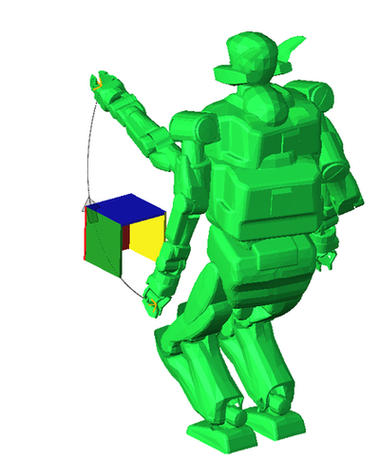
\includegraphics[width = \columnwidth]
                    {src/chap3-optimal-motion-planning/figure/simple-path.png}
    \caption{Initial invalid path.}
    \label{simple-path}
  \end{subfigure}
  \begin{subfigure}{0.32\columnwidth}
    \centering
    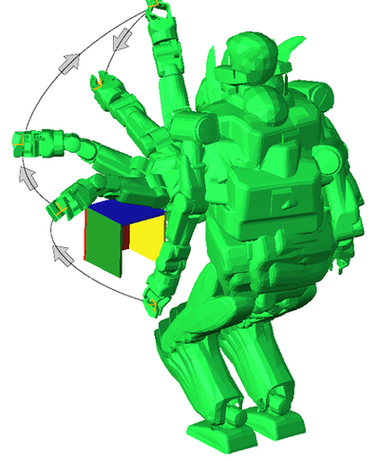
\includegraphics[width = \columnwidth]
                    {src/chap3-optimal-motion-planning/figure/simple-path-sol.png}
    \caption{RRT path.}
    \label{simple-path-sol}
  \end{subfigure}
  \begin{subfigure}{0.32\columnwidth}
    \centering
    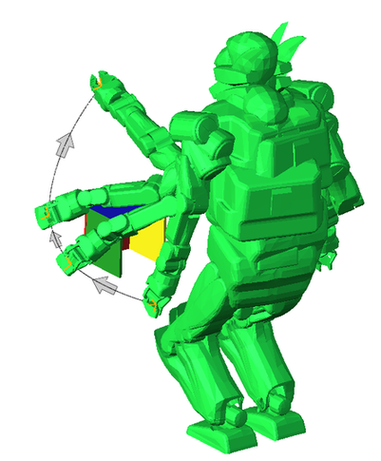
\includegraphics[width = \columnwidth]
                    {src/chap3-optimal-motion-planning/figure/simple-path-sol-shortcut.png}
    \caption{Shortcut path.}
    \label{simple-path-sol-shortcut}
  \end{subfigure}
  \caption{Paths for the test case.}
\end{figure}

We demonstrate the effectiveness of our optimal motion planning
framework by first using it in a a simple test case example, then
applying it to generate feasible motions on the robot HRP-2. All tests
were run on a computer with a 2.53 GHz
Intel\textsuperscript{\textregistered} Core\texttrademark2 Duo
processor.

\subsection{Test Case}
\label{test-case}
Figure \ref{simple-path} shows the motion planning problem to be
solved: HRP-2 starts from its rest position and moves to a goal
configuration by raising its left arm. A concave object is placed such
that the left hand is at one point enclosed in it if the initial path
connecting the start to goal configuration is executed. This is a
typical example of a problem with a local minimum defined by the
environment, where a real-time control approach in task-space might
fail. Figure \ref{simple-path-sol} shows a possible solution path
found with constrained RRT. This path can be shortened with a shortcut
optimizer, as in figure \ref{simple-path-sol-shortcut}.

To showcase the usefulness of our approach, we try to solve the
optimal control problem defined in Section \ref{framework} starting
from the different paths, and put all results in Table
\ref{table}. When starting with the initial path from figure
\ref{simple-path}, the solver failed to achieve a single
iteration. This can be explained by the fact that in the middle of
this path, the robot left hand is enclosed inside the obstacle and
some distance constraints are violated; the solver fails to determine
a clear direction which would remove this violation due to the
geometric local minimum. Since the constrained RRT avoids it and
generates a collision-free path, the solver behaves correctly when
starting with the path in \ref{simple-path-sol}, but the maximum
number of iterations is reached before reaching convergence. It is
achieved when starting with the shortcut path in
\ref{simple-path-sol-shortcut}. Note that about 70\% of the
optimization time is spent in evaluating the distance constraints and
their gradients; this significant overhead can be explained by the
fact that \textsc{MUSCOD-II} relies on internal numerical
differentiation to compute Jacobians. Relying on analytical gradient
expressions would thus accelerate the optimization process. Regarding
the distance constraints enforcement, figure
\ref{simple-distance-constraints} shows the evaluation of the left arm
distances: due to the constraints time discretization, one constraint
is violated during less than 100ms. This violation does not however
exceed 4mm, and this is considered as acceptable as all distance
constraints are computed with bounding capsule geometries which
already define conservative volumes around the exact geometries.

\begin{table}
  \renewcommand{\arraystretch}{1.3}
  \caption{Test Case Computation Times}
  \label{table}
  \centering
  \begin{tabular}{|c||c|c|c|}
    \hline
    Initial guess & Initial path & RRT path & Shortcut path \\
    \hline
    Planning time (s) & -- & 5 & 5 \\
    \hline
    Shortcut time (s) & -- & -- & 4 \\
    \hline
    Optimization status & ERROR & MAX\_ITER & OK \\
    \hline
    SQP iterations & -- & 200 & 70 \\
    \hline
    Optimization time (s) & -- & 3068 & 1186 \\
    \hline
    Constraints evaluation time (s) & -- & 2176 & 847 \\
    \hline
  \end{tabular}
\end{table}

FIXME: remove figure and plot from data instead? or use matplotlib to
make nicer plot.

\begin{figure}
  \centering
  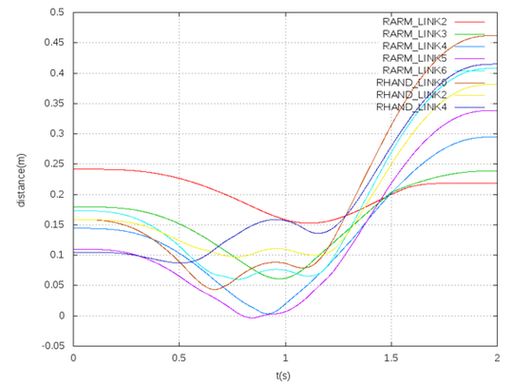
\includegraphics[width=0.8\linewidth]
                  {src/chap3-optimal-motion-planning/figure/distance-constraints.png}
  \caption{Plots of left arm body distance constraints.}
  \label{simple-distance-constraints}
\end{figure}

\subsection{Fast Trajectory Generation on HRP-2}

We also use our approach to generate fast optimal collision-free
trajectories and execute them on the humanoid robot HRP-2. In the
first scenario, HRP-2 executes a kind of martial art figure where it
crosses its arms rapidly while bending its knees, changes the arms
configuration, then moves back to a rest posture. The motion must be
executed while ensuring the arms do not collide with each other, and
the robot does not fall. This is quite a difficult task as the 3
trajectories durations are fixed to 1, 2, and 2 seconds
respectively. Particularly, the second motion where one arm goes from
being behind the other arm to being ahead of it proved to be
impossible to generate without a prior planning phase as proposed in
out approach.

In the second scenario, we add a complex environment that contains
shelves with different levels; HRP-2 first bends its knees to grab a
ball located deep on the lower shelf, then moves it to an upper shelf
to release it between two other objects. The trajectories last
respectively 2 and 5 seconds. Here, both collision and self-collision
constraints need to be enforced in order to obtain a valid
trajectory. Again, the ball transfer motion cannot be generated using
an optimal control solver and a simple initial guess; a prior planning
phase is needed to find a collision-free transfer path.

We successfully apply our framework to generate feasible motions for
both scenarios as seen in figures \ref{self-collision} and
\ref{shelves}. Computation times are shown in Tables
\ref{table-martial-art} and \ref{table-shelves}. Videos of both
scenarios are available in the attached file.

\begin{figure}
  \centering
  \begin{subfigure}{0.19\columnwidth}
    \centering
    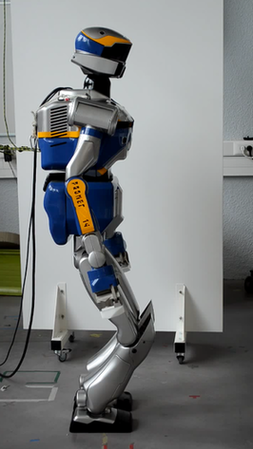
\includegraphics[width = \columnwidth]
                    {src/chap3-optimal-motion-planning/figure/self-collision-1.png}
    \label{self-collision-1}
  \end{subfigure}
  \begin{subfigure}{0.19\columnwidth}
    \centering
    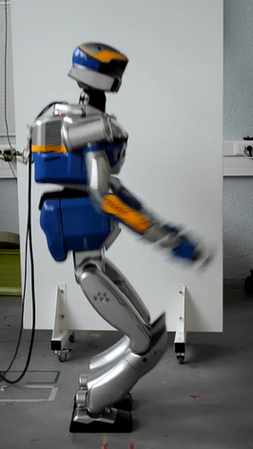
\includegraphics[width = \columnwidth]
                    {src/chap3-optimal-motion-planning/figure/self-collision-2.png}
    \label{self-collision-2}
  \end{subfigure}
  \begin{subfigure}{0.19\columnwidth}
    \centering
    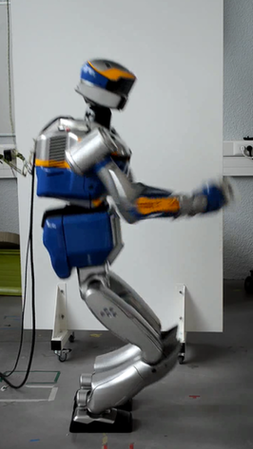
\includegraphics[width = \columnwidth]
                    {src/chap3-optimal-motion-planning/figure/self-collision-3.png}
    \label{self-collision-3}
  \end{subfigure}
  \begin{subfigure}{0.19\columnwidth}
    \centering
    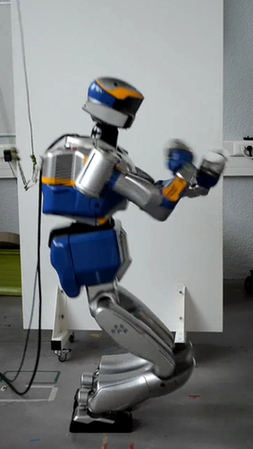
\includegraphics[width = \columnwidth]
                    {src/chap3-optimal-motion-planning/figure/self-collision-4.png}
    \label{self-collision-4}
  \end{subfigure}
  \begin{subfigure}{0.19\columnwidth}
    \centering
    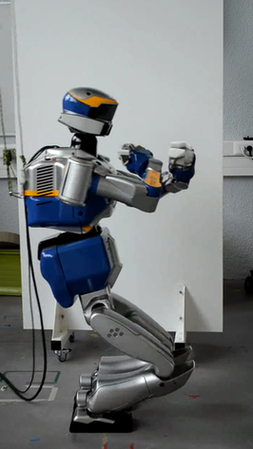
\includegraphics[width = \columnwidth]
                    {src/chap3-optimal-motion-planning/figure/self-collision-5.png}
    \label{self-collision-5}
  \end{subfigure}
  \begin{subfigure}{0.19\columnwidth}
    \centering
    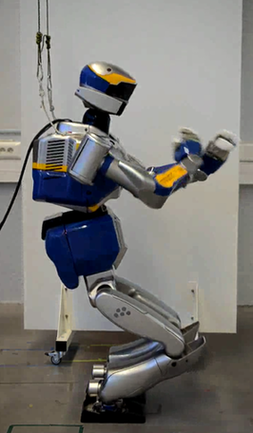
\includegraphics[width = \columnwidth]
                    {src/chap3-optimal-motion-planning/figure/self-collision-6.png}
    \label{self-collision-6}
  \end{subfigure}
  \begin{subfigure}{0.19\columnwidth}
    \centering
    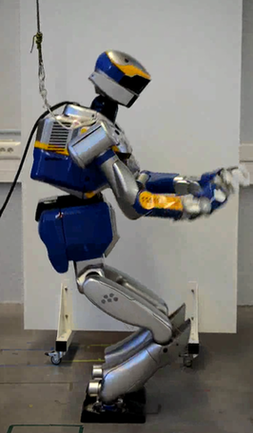
\includegraphics[width = \columnwidth]
                    {src/chap3-optimal-motion-planning/figure/self-collision-7.png}
    \label{self-collision-7}
  \end{subfigure}
  \begin{subfigure}{0.19\columnwidth}
    \centering
    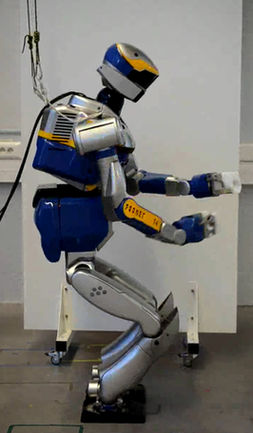
\includegraphics[width = \columnwidth]
                    {src/chap3-optimal-motion-planning/figure/self-collision-8.png}
    \label{self-collision-8}
  \end{subfigure}
  \begin{subfigure}{0.19\columnwidth}
    \centering
    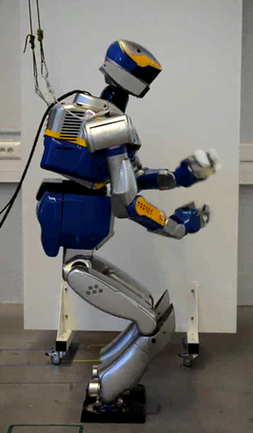
\includegraphics[width = \columnwidth]
                    {src/chap3-optimal-motion-planning/figure/self-collision-9.png}
    \label{self-collision-9}
  \end{subfigure}
  \begin{subfigure}{0.19\columnwidth}
    \centering
    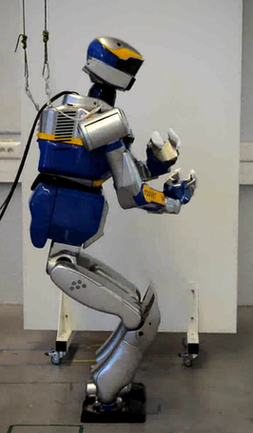
\includegraphics[width = \columnwidth]
                    {src/chap3-optimal-motion-planning/figure/self-collision-10.png}
    \label{self-collision-10}
  \end{subfigure}
  \caption{HRP-2 does a quick martial arts motion while avoiding
    self-collision.}
  \label{self-collision}
\end{figure}

\begin{figure}
  \centering
  \begin{subfigure}{0.19\columnwidth}
    \centering
    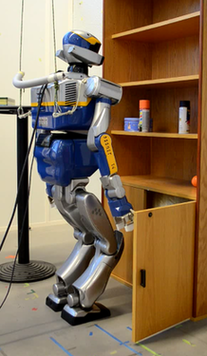
\includegraphics[width = \columnwidth]
                    {src/chap3-optimal-motion-planning/figure/shelves-1.png}
    \label{shelves-1}
  \end{subfigure}
  \begin{subfigure}{0.19\columnwidth}
    \centering
    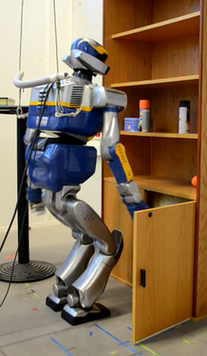
\includegraphics[width = \columnwidth]
                    {src/chap3-optimal-motion-planning/figure/shelves-2.png}
    \label{shelves-2}
  \end{subfigure}
  \begin{subfigure}{0.19\columnwidth}
    \centering
    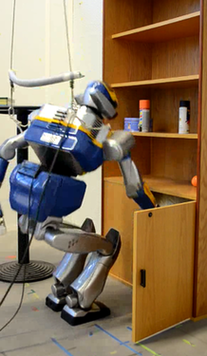
\includegraphics[width = \columnwidth]
                    {src/chap3-optimal-motion-planning/figure/shelves-3.png}
    \label{shelves-3}
  \end{subfigure}
  \begin{subfigure}{0.19\columnwidth}
    \centering
    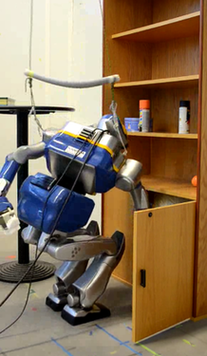
\includegraphics[width = \columnwidth]
                    {src/chap3-optimal-motion-planning/figure/shelves-4.png}
    \label{shelves-4}
  \end{subfigure}
  \begin{subfigure}{0.19\columnwidth}
    \centering
    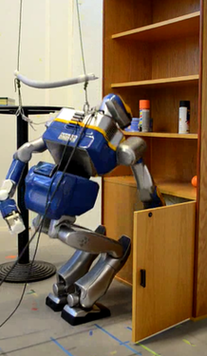
\includegraphics[width = \columnwidth]
                    {src/chap3-optimal-motion-planning/figure/shelves-5.png}
    \label{shelves-5}
  \end{subfigure}
  \begin{subfigure}{0.19\columnwidth}
    \centering
    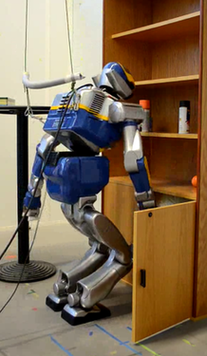
\includegraphics[width = \columnwidth]
                    {src/chap3-optimal-motion-planning/figure/shelves-6.png}
    \label{shelves-6}
  \end{subfigure}
  \begin{subfigure}{0.19\columnwidth}
    \centering
    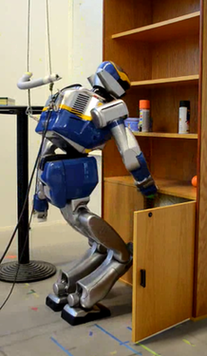
\includegraphics[width = \columnwidth]
                    {src/chap3-optimal-motion-planning/figure/shelves-7.png}
    \label{shelves-7}
  \end{subfigure}
  \begin{subfigure}{0.19\columnwidth}
    \centering
    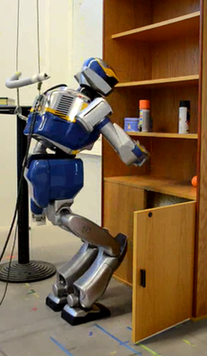
\includegraphics[width = \columnwidth]
                    {src/chap3-optimal-motion-planning/figure/shelves-8.png}
    \label{shelves-8}
  \end{subfigure}
  \begin{subfigure}{0.19\columnwidth}
    \centering
    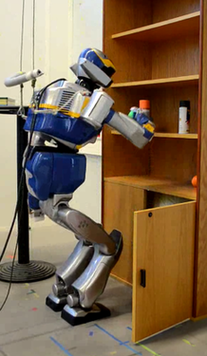
\includegraphics[width = \columnwidth]
                    {src/chap3-optimal-motion-planning/figure/shelves-9.png}
    \label{shelves-9}
  \end{subfigure}
  \begin{subfigure}{0.19\columnwidth}
    \centering
    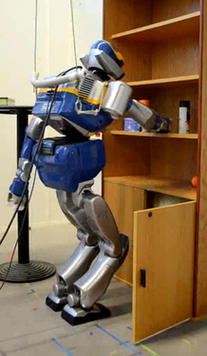
\includegraphics[width = \columnwidth]
                    {src/chap3-optimal-motion-planning/figure/shelves-10.png}
    \label{shelves-10}
  \end{subfigure}
  \caption{HRP-2 bends down quickly to grab a ball in the lower
    shelf and transfers it to the upper shelf.}
  \label{shelves}
\end{figure}

\begin{table}
  \renewcommand{\arraystretch}{1.3}
  \caption{Computation Times for Martial Arts Scenario}
  \label{table-martial-art}
  \centering
  \begin{tabular}{|c||c|c|c|}
    \hline
    Phase & 1 & 2 & 3 \\
    \hline
    Planning time (s) & 4 & 13 & 2 \\
    \hline
    Shortcut time (s) & 4 & 6 & 1 \\
    \hline
    SQP iterations & 32 & 73 & 25 \\
    \hline
    Optimization time (s) & 346 & 1130 & 278 \\
    \hline
    Constraints evaluation time (s) & 124 & 356 & 83 \\
    \hline
  \end{tabular}
\end{table}

\begin{table}
  \renewcommand{\arraystretch}{1.3}
  \caption{Computation Times for the Shelves Scenario}
  \label{table-shelves}
  \centering
  \begin{tabular}{|c||c|c|}
    \hline
    Phase & 1 & 2 \\
    \hline
    Planning time (s) & 13 & 38 \\
    \hline
    Shortcut time (s) & 6 & 23 \\
    \hline
    SQP iterations & 74 & 80 \\
    \hline
    Optimization time (s) & 1745 & 5020 \\
    \hline
    Constraints evaluation time (s) & 1396 & 2640 \\
    \hline
  \end{tabular}
\end{table}

\subsection{Discussion}
\label{discussion}

In subsection \ref{test-case}, we demonstrate in a simple example the
influence of the initial guess of the optimal control problem on the
solver success and performance. In fact, due to its probabilistic
completeness, the usage of the constrained planner in a first stage
guarantees that an initial collision-free and quasi-statically
feasible trajectory can be found. The optimization solver then can
reshape this trajectory in order to minimize the objective function
while enforce constraints such as joint limits and dynamic
balance. Note that with this method, locally optimal trajectories are
found; in order to find global optima, it might be interesting to plan
in \cspace\thinspace using RRT* instead of RRT in the first stage.

The trajectory duration is for the moment fixed. This means that if it
is not properly set, the optimization solver might fail as some
constraints such as velocity limits would never be enforced. If it is
included as a free variable in the optimal control problem, we will
have a guarantee of success for the second stage. The complete
framework would then always succeed in generating optimal
trajectories.

\section{Conclusion}
In this paper we propose a novel approach to tackle optimal control
problems in cluttered environments. Our approach combines, in a
two-stage framework, a constrained path planning algorithm and an
optimal control problem solver. We generate optimal feasible
trajectories for the humanoid robot HRP-2 and successfully execute
them.

Our framework can benefit from improvements to increase its
usability. Future work will consider non-coplanar contacts, as well as
release the robot from its fixed support constraints in order to
accomplish optimal locomotion planning.
